\documentclass[twocolumn, 10pt,a4j]{jsarticle}
  \usepackage{here}
  \usepackage{amsmath}
  \usepackage[dvipdfmx]{graphicx}
  \usepackage{url}
  % プリアンブル
  \title{\vspace{-2.5cm}振動の計測と制御}
  \author{1610581 堀田 大地}
  \date{2018/7/26}
  \begin{document}
  \maketitle{}
  \section{結果}
    各周波数での結果画像を図6,7,8,9に,結果の値を表2に示した.表2より,$dy$が最も大きくなるのは40Hzのときなので,40Hzが共振周波数である.
    \begin{table}[]
      \centering
        \caption{周波数Hzと$dx mS, dy V$の関係}
        \label{my-label}
        \footnotesize
        \begin{tabular}{llll}
          周波数Hz V & $dx$ mV & $dy$ V & $\frac{dy}{周波数}$  \\ \hline
          20 & 23.804 & -16.649 & 1.129 \\
          40 & -12.939 & -51.138 & 1.145 \\
          60 & 7.751 & -24.817 & 1.020 \\
          80 & 5.920 & -20.800 & 0.9616 \\
          100 & 5.615 & -20.615 & 1.074 \\
        \end{tabular}
      \end{table}

    \begin{figure}[H]
      % 図6
      \begin{center}
        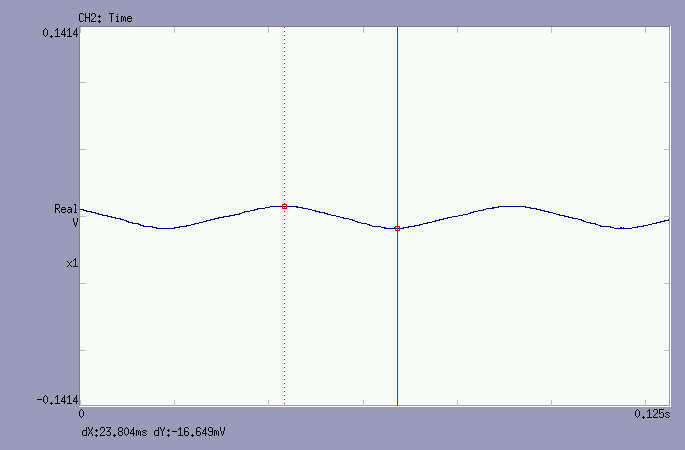
\includegraphics[width=7cm]{../img/experiments/006.png}
        \caption{周波数20Hz}
      \end{center}
    \end{figure}

    \begin{figure}[H]
      % 図1
      \begin{center}
        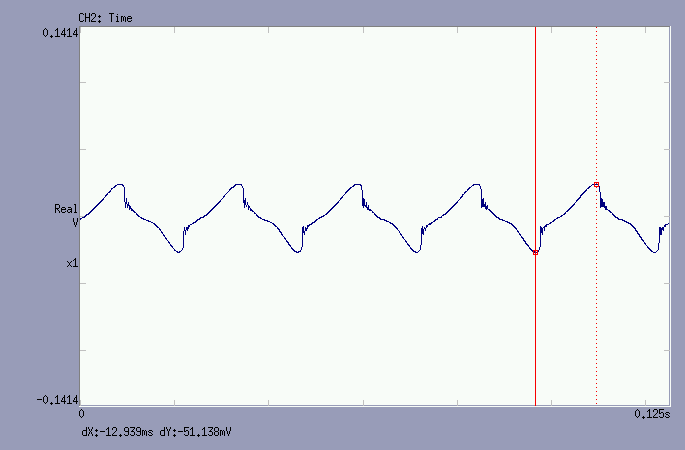
\includegraphics[width=7cm]{../img/experiments/007.png}
        \caption{周波数40Hz}
      \end{center}
    \end{figure}

    \begin{figure}[H]
      % 図1
      \begin{center}
        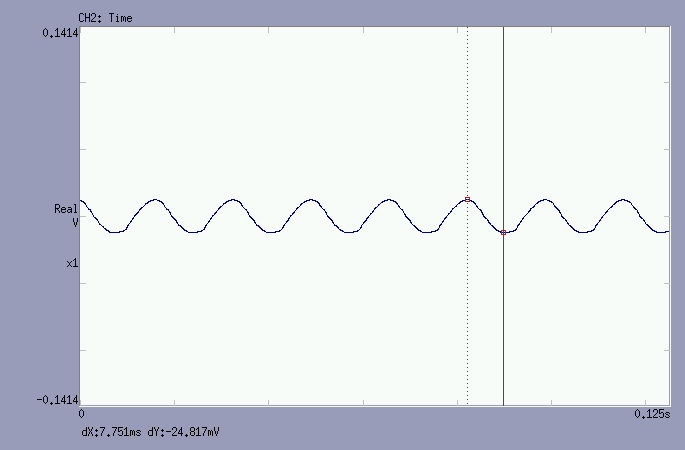
\includegraphics[width=7cm]{../img/experiments/008.png}
        \caption{周波数60Hz}
      \end{center}
    \end{figure}

    \begin{figure}[H]
      % 図1
      \begin{center}
        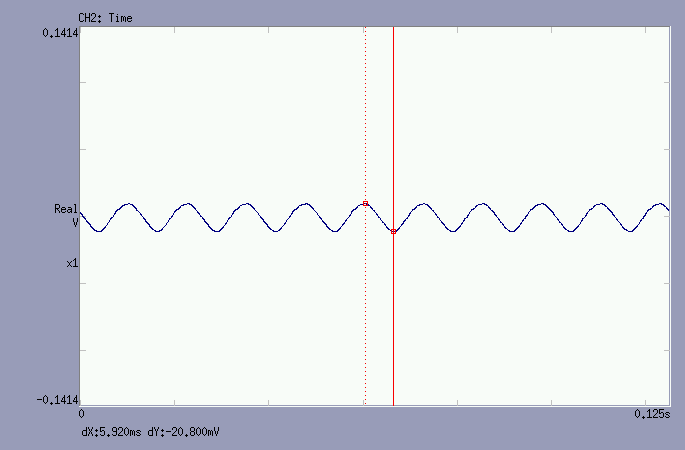
\includegraphics[width=7cm]{../img/experiments/009.png}
        \caption{周波数80Hz}
      \end{center}
    \end{figure}

    \begin{figure}[H]
      % 図10
      \begin{center}
        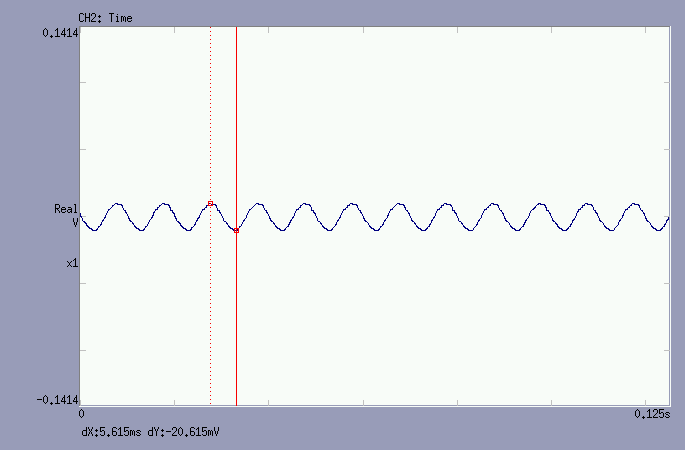
\includegraphics[width=7cm]{../img/experiments/010.png}
        \caption{周波数100Hz}
      \end{center}
    \end{figure}
  \end{document}